\section{}

\begin{figure}
    \begin{center}
    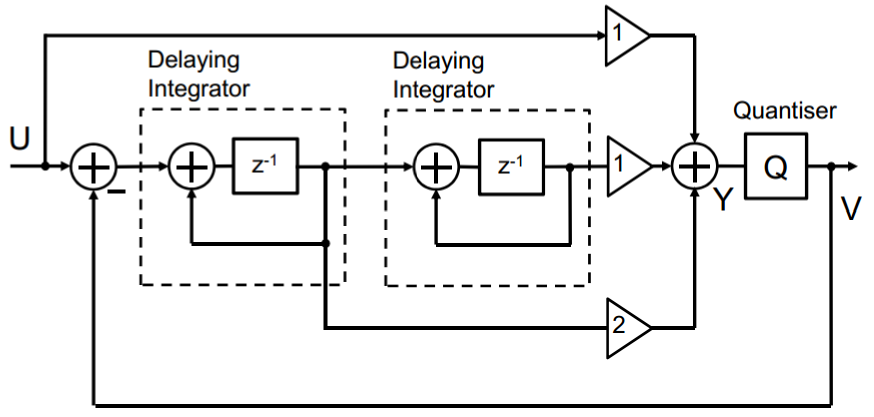
\includegraphics[width=0.8\textwidth]{silvasteensgard.png}
    \caption{A Silva-Steensgard second order modulator diagram.}
    \label{fig:silva}
    \end{center}
\end{figure}
%this question should focus on deriving the quantisation noise power in second order converter
    \subsection{}
    %derive STF ans NTF
    Derive the STF and NTF for the modulator shown in figure \ref{fig:silva}.

    %STF is just 1, looks like
    %NTF is (1-z^{-1})^{2}

    %start with deriving the NTF, then go from there

    \subsection{}
    %then derive the quantisation noise power from this?
    What is the expression describing the quantisation noise power in this modulator?

    %will put answers here when I've done them

    \subsection{}
    %then the SQNR
    With a signal amplitude of M, what is the expected SQNR of this modulator?

    %will put answers here when I've done them
